\documentclass[tikz]{standalone} 

\usepackage{newtxtext,newtxmath}

\input{mytikzset}
\definecolor{myGreen}{RGB}{0,127,0}

\begin{document}
\nopagecolor
  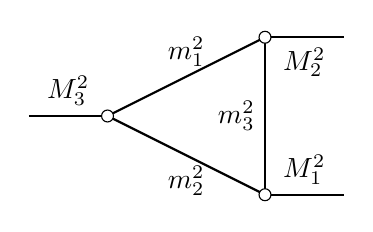
\begin{tikzpicture}[node distance=0.6cm and 0.9cm, baseline=1cm]
    \draw[thick]  (0,0) -- node[above] {$M_3^2$} (1,0);
    \draw[thick]  (1,0) -- node[above] {$m_1^2$} (3,1);
    \draw[thick]  (1,0) -- node[below] {$m_2^2$} (3,-1);
    \draw[thick]  (3,-1) -- node[left] {$m_3^2$} (3,1);
    \draw[thick]  (3,-1) -- node[above] {$M_1^2$} (4,-1);
    \draw[thick]  (3,1) -- node[below] {$M_2^2$} (4,1);

    \draw[black, fill=white] (1,0) circle (0.5ex);
    \draw[black, fill=white] (3,1) circle (0.5ex);
    \draw[black, fill=white] (3,-1) circle (0.5ex);
  \end{tikzpicture}
\end{document}
